\section{Introduction}

The goal of this paper, an effective metric for computing distance between program executions (in particular, failing test cases), is motivated in large part by progress in automated testing.  Recent advances, some implemented in powerful tools \cite{csmith,jsfunfuzz,ISSTA12,LangFuzz,ZhendongPLDI,ZhendongOOPSLA}, have made it easier to find subtle faults in, e.g., modern optimizing compilers\footnote{In this paper, we take the problem of testing and debugging compilers as representative of the general problem of testing and debugging complex critical systems software.}.  Unfortunately, the blessing of many failing test cases can become a curse for a developer.  Simply discovering which test cases in a large set of failures represent distinct faults (or already known faults) is a very difficult problem \cite{PLDI13,Podgurski04}.  For simple crashes and assertion violations, bucketing failures is sometimes easy.  When a failure is detected by differential testing \cite{Differential}, where two compilers or optimization levels disagree, the problem is so hard that it may turn potential users away from automated test generation \cite{PLDI13}.  Even once a fault is identified, fixing the problem can be very difficult.  Due to complexity of intermediate representation, interaction of optimizations, subtle language semantics, and other issues, debugging compiler faults may often be harder than debugging faults in other kinds of software (this is probably not limited to compilers; debugging systems software in general is hard \cite{mickens}).
We propose the use of program mutants \cite{mutant} to assist debugging based on large sets of automatically generated test cases.  The underlying idea is that if two failures can be repaired in the same way, even if that repair only avoids the failure and does not truly fix it, they are likely due to the same fault. Repairs can also provide  information for understanding and debugging discovered faults. The approach suggests a plausible metric for comparing any two program executions, not just failing test cases.

\subsection{Fuzzer Taming and Debugging Assistance}

Automated test generators tend to produce many failures, which correspond to far fewer faults.  The distribution of faults in a set of failures tends to follow a strong power-law curve, where a few faults account for most failures, and many or even most faults have only 1 or 2 associated failures (even in a set of 1,000 or more test cases) \cite{PLDI13}.  Looking at all the failures to find  distinct faults is impractical.  It is also impractical to apply the iterative approach:  first, fix one fault; then re-run all tests, knowing that the remaining failures are due to unfixed faults, repeating until all tests pass.  There may be some (possibly known) faults that are very difficult to fix. As of 11/20/2015, LLVM clang had 89 bugs assigned but not resolved, some dating to 2008.  Knowing if a randomly generated test case is an instance of a known failure can be difficult, and fixing these problems is unlikely.    A research group with a novel fault-detection technique \cite{csmith,ISSTA12,ZhendongPLDI} may dump dozens of new faults on a project at once, producing more open problems.   High priority faults may be hidden by stubborn low-priority faults.

In a PLDI 2013 paper, Chen et al. defined the \emph{fuzzer taming problem}: ``Given a potentially large collection of test cases, each of which triggers a bug, rank them in such a way that test cases triggering distinct bugs are early in the list.'' \cite{PLDI13}.  Their proposed solution was to use the Furthest-Point-First \cite{Gonzalez} (FPF) algorithm.  An FPF ranking of test cases requires a distance metric $d$ on test cases, and ranks test cases so that dissimilar tests appear earlier.  The hypothesis of Chen et al. was that dissimilar tests, by a well-chosen metric, will also fail due to different faults.
FPF is a greedy algorithm that proceeds by repeatedly adding the item with the maximum minimum distance to all previously ranked items. Given an initial seed item $r_0$, a set
$S$ of items to rank, and a distance metric $d$, FPF computes $r_i$ as $s \in S: \forall s' \in S: min_{ j < i}(d(s,r_j)) \geq min_{j < i}(d(s',r_j))$.

Fuzzer taming results using FPF were promising, but limited.  Rather than proposing a universal metric for use in fuzzer taming, Chen et al. offered many possible metrics (based on ideas in the literature, such as edit distances \cite{lev} or coverage spectra \cite{RepsSpectra} methods), none of which performed notably well across all three benchmark data sets, and some of which were not even applicable to all data sets.  For the two most difficult benchmarks, none of the metrics performed extremely well. FPF-based approaches remain in need of a universal but effective metric, particularly for the critical first 50 test cases examined \cite{PLDI13}.

One reason fuzzer taming is needed is that debugging compiler faults is, as noted, difficult.  If developers were able to fix faults quickly once they were identified, it would not be as important to have very good fault identification.  Many duplicate failures could be removed by fixing the underlying faults.  Ideally, a technique able to provide effective fuzzer taming should be able to translate its underlying rationale into some form of automated debugging assistance.   A variety of automated debugging methods \cite{NearNeighbor,GroceError} have been based on distance, so there is reason to expect that a high-quality metric might also contribute to fault localization.

\subsection{Comparing Executions by Response to Mutation}

The key insight of this paper is a hypothesis with numerous possible applications, including a universal fuzzer taming metric that can also provide assistance in debugging.  

\begin{quote}
{\bf Hypothesis 1:} If two test cases that fail can be made to succeed by the same syntactic modification to the original program $P$, this provides evidence that they fail due to the same fault.
\end{quote}

The core idea is hardly controversial:  most developers determine if they have fixed all faults in a set of failing test cases by re-running the tests after they fix at least one fault.  As a method for fuzzer taming or debugging assistance, however, this is useless.  Fortunately, developer-provided patches are not the only source of syntactic changes to a program.  Mutation analysis \cite{demillo1978hints,budd1980theoretical} applies large numbers of syntactic changes to a program, usually to evaluate a test suite \cite{mutant,justmutants}.  Some recent work has also considered these changes as a source of fixes or localizations for program faults \cite{achour,multilingual,MUSE,DebroyMutant}.  Our experience, as well as empirical data \cite{GopinathMutants}, suggests that very few compiler faults are due to the kind of simple syntactic changes found in mutants.  However, this does not matter for {\bf Hypothesis 1};  what matters is that failures, which correspond to faults, can be made to succeed.  When a test case $t$ fails for program $P$ but succeeds for mutant $m$ of $P$ we say that $m$ \emph{repairs} $t$.  In most cases this does not mean that $m$ is the inverse of a fault, but that $m$ somehow avoids the consequence of a fault.  It is not important that repairs actually fix anything, if all we seek is a way to decide whether failures are due to the same fault.

Hypothesis 1 is in fact a consequence of a more general (and difficult to investigate) hypothesis.  What is interesting about a program execution?  For many purposes, the only interesting properties of an execution are those that in some way relate to the correctness properties of the program, assuming we have a good set of correctness properties.  These may include assertions, differential testing \cite{Differential,ICSEDiff}, timing constraints, temporal logic formulas, or any other checkable properties.  What, then, makes two executions similar?  Our proposal is to say that:

\begin{quote}
{\bf Hypothesis 2:} Two executions of $P$ are similar to the degree that changes to $P$ produce the same changes in correctness of the executions.
\end{quote}

This leads to the idea of comparing executions by their response to mutants.   In the presence of multiple correctness properties, any two executions can be compared, not just two failures, since a mutant can cause a failure to violate additional or different properties.
%Where there are multiple, independent, correctness properties, this even allows us to compare failing and successful executions, since a mutant can cause a failure to violate a different property.
{\bf Hypothesis 2} at first may suggest that this idea subsumes past notions of similarity, such as spectra of code coverage, since if two executions do not cover a statement, they both cannot alter correctness if that statement is altered.  The metrics are in fact simply incomparable:  for example, differences in coverage that never have an effect on correctness cannot contribute to similarity in our approach; with weak correctness properties most executions are very similar.  This is similar to the idea of \emph{checked coverage}:  code that cannot impact correctness is not interesting \cite{CheckCov}.  Hypothesis 2 also suggests an additional hypothesis related to hypothesis 1.  This is {\bf Hypothesis 1a:} If two failing test cases can be made to differ as to whether they fail by a modification of $P$, this provides evidence that they fail due to different faults.

\subsection{The Onion-Ring and Causality}

These hypothesis do not claim that being repaired by the same mutant perfectly predicts fault equivalence.  To understand why that seems highly unlikely, consider why a mutant of a compiler might cause a test case to stop failing.  Many, likely most, compiler faults are due to incorrect optimizations.  Turning an optimization off can cause a program to compile correctly.  Optimizations are generally guarded by conditional switches --- in some cases, so that the optimization can be turned off by a user, in other cases when a property of the code in question prevents the optimization.  If two failures become successes due to turning off an optimization, it is certainly some level of evidence they are the same fault, compared to the baseline probability.  Intuitively, the evidence provided seems much stronger than the fact that, e.g., the two test cases execute a shared line of code \cite{RepsSpectra}.  However, optimization guards range from guarding very specific fragments of code to guarding entire modules with many functions and related sub-optimizations.  If a mutant prevents a very specific optimization (consisting of a few lines of code) from executing, and repairs two tests, that is powerful evidence they are related.  If a mutant turns off a large number of optimizations, it is weak evidence.  Characterizing the granularity of program mutants is likely difficult, but fortunately it is not necessary.

\begin{figure}
\centering
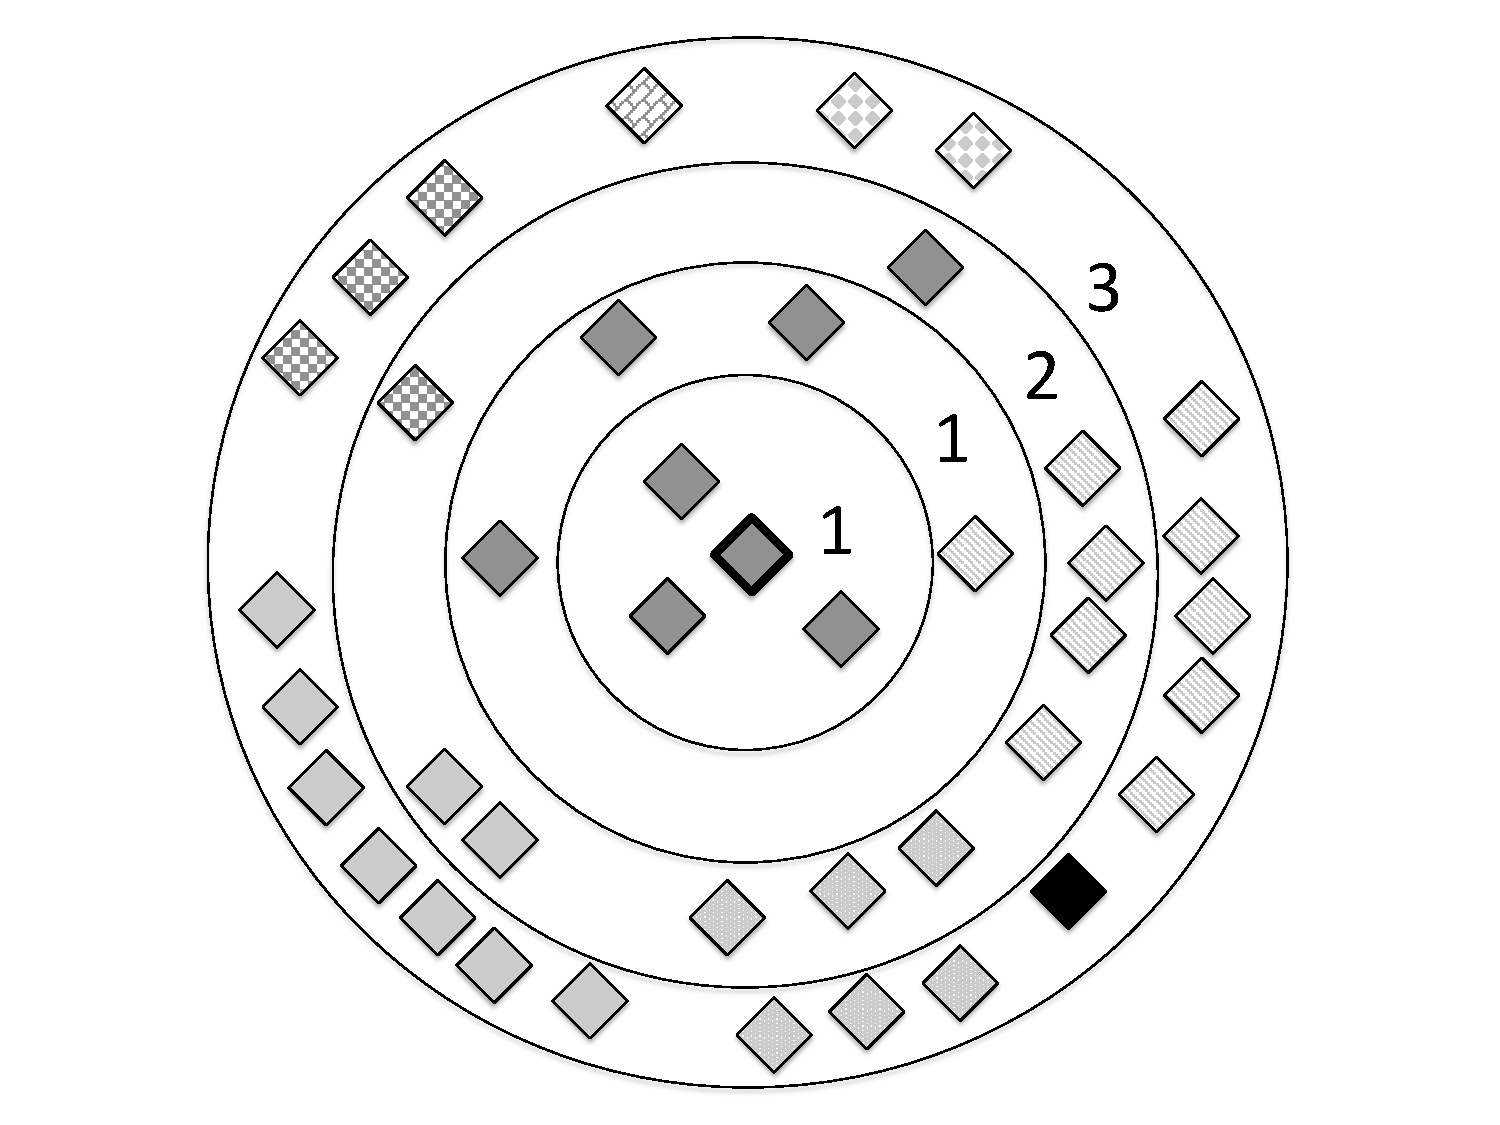
\includegraphics[width=0.6\columnwidth]{onionring}
\caption{\scriptsize{The onion-ring model of repairs, showing all repairs for the center-most test case, and all other test cases repaired by those mutants.  Circles represent repairing mutants, and diamonds repaired test cases.  Diamond pattern symbolizes fault.  For the innermost ring of repairing mutant(s), all test cases are due to the same fault.  As rings expand to include more failures, the set of faults repaired grows (as does distance).}}
\label{fig:onion}
\end{figure}

Consider the structure of mutants repairing a failure due to some optimization.  If many mutants repair this failure, by turning off the optimization or a whole family of optimizations, some will likely repair failures due to different faults.  Repairs naturally produce an \emph{onion-ring} structure (Figure \ref{fig:onion}), where a failure is repaired by (1) some mutants that are very specific to its fault (the inner rings) and repair few failures, as well as other mutants (2) that repair more and more faults, up to a hypothetical mutant (3) that turns off all optimization in the compiler (e.g., by effectively adding {\tt -O0}), the outer ring of the onion.  This does not introduce confusion, because the more repairs two tests have in common, the more likely they are to be due to the same fault, and the more they disagree on, the less likely they are to be due to the same fault.  While especially intuitive as a consequence of disabling compiler optimizations, it seems likely this structure appears for repairs in many programs.  Disabling an optimization is a code change that (usually) does not cause any test case that only concerns semantics, not speed, to fail, but can avoid some failures.  For some oracles, many changes may fall into this classification:  for example, if the only oracle is to detect crashes, a fault can be avoided by aborting the program early.  Turning off a data-structure invariant checker is another possible false repair that might cover many different faults.  In all these cases, so long as there are other, more interesting and more specific ways to repair some faults, a distance metric can still distinguish faults effectively.

The idea of measuring the distance between failures (or other test cases) by their response to mutants is appealing.  The most important aspect of most applications of distances between executions is some aspect of causality \cite{LewisCause,ZellerBook}.  Since at least the work of Hume \cite{Hume1}, causality has been understood as answering some question of the form ``what would have made a difference in this effect?''  A program mutant is a very direct way to answer this question.  The problem with determining causes of events in computer programs is that, as in most problems of causality, too many things can make a difference, most of which are not interesting.  Program mutants are much more likely to be interesting causes for events in a program than changes to test cases, at least for fault identification and debugging purposes, because the practical use of knowing a cause is to change the cause and avoid or produce an effect.  Debugging by changing test cases is not useful; debugging by altering the program is precisely how we seek to use the causes we discover.  Using mutants as causes in order to measure similarity essentially inverts the ideas of David Lewis \cite{LewisCause,LewisCount}, where similarity is used to determine causality.  

\subsection{Contributions}

The contributions of this paper are: hypotheses about how to measure distance between program executions, and practical proposals for using such a metric in fuzzer taming and in novel fault localization and explanation methods.  Evaluating the effectiveness of these methods also provides experimental evidence as to the validity of our hypotheses.  Our experimental results show that, for two realistic complex compilers, Mozilla's SpiderMonkey 1.6 JIT for JavaScript and GCC 4.3.0, using mutant response metrics improves FPF-based fuzzer taming over previous results \cite{PLDI13}, in multiple ways.  Our preliminary localization approaches compare favorably to state-of-the-art fault localization techniques \cite{MUSE,multilingual}, for the mutation analysis budget in our experiments.